\documentclass{article}
\usepackage{iclr2016_conference,times}

\usepackage{subfig}
\usepackage{float}
\usepackage{hyperref}
\usepackage{url}
\usepackage{amsmath,amssymb}
\usepackage{natbib}
\usepackage{wrapfig}
\usepackage{graphicx}
\usepackage{soul}
\bibliographystyle{abbrvnat}

\title{
	Mobile Computing (CS23400$/$1) \vspace{-4pt} \\
	{\Large Lab 1 - Report} \vspace{6pt} \\
	{\large Andrea F. Daniele $\hspace{2.2cm}$ Max X. Liu $\hspace{2.2cm}$ Noah A. Hirsch}
}

\begin{document}

\maketitle


\vspace{-1.2cm}

\section{Task}
\vspace{-.3cm}
The goal of this lab is to collect and leverage IMU data from a small robotic
car to classify a set of activities. Using the IMU data we can implement machine
learning models to classify IMU traces into four distinct activities (walking,
jumping, standing, driving). Furthermore, the classification model used should
be robust to challenges with low quality IMU's and mobile computation limits.

\section{Challenges}
\vspace{-.3cm}
One of the primary challenges faced was extracting consistent and relevant data
from the IMU traces. Due to imperfect measurements from the IMU, the raw data
contains a lot of noisy readings that complicate the problem of classifying
activities. Furthermore, it is very computationally intensive to train Recurrent
Neural Networks with such large trace files; additional pre-processing of data
is necessary to help train the model. An additional concern was that there may
not be enough data and/or features to effectively train a Recurrent Neural Network.

\section{Proposed Approach}
\vspace{-.3cm}

This task belongs to the family of classification tasks, extensively studied in applied machine
learning. In particular, it belongs to the subfamily of \textbf{sequence labeling} tasks, in which
a stream of feature vectors of length $T$ is assigned a single label picked among a set of valid
labels.

\begin{wrapfigure}{r}{0.28\textwidth}
    \centering
    \vspace{-8pt}
    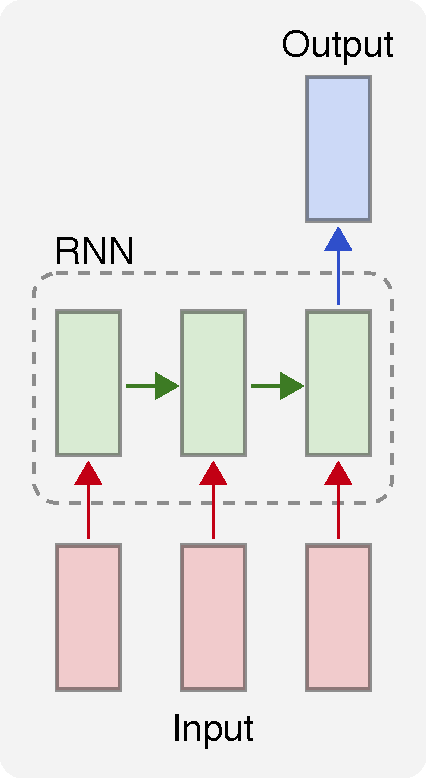
\includegraphics[width=0.24\textwidth]{figures/rnn}
    \caption{RNN Architecture known as Many-to-One \label{fig:rnn}}
    \vspace{-12pt}
\end{wrapfigure}

Different approaches have been proposed for both temporal and non-temporal sequences.
The state-of-the-art architecture for classifying temporal sequences is called Recurrent Neural
Network (RNN). Unlike classic feedforward neural networks, RNNs can use their internal memory
to process arbitrary sequences of inputs. Their internal memory also allows them to remember
features vectors received at previous time instants which make them very effective in classifying
temporal sequences.

One of the main problems with RNNs is the so-called vanishing gradient problem. In particular,
during the training phase, the gradient that is back-propagated from the last RNN (right-most
RNN in Fig.~\ref{fig:rnn}) towards the first RNN (left-most RNN in Fig.~\ref{fig:rnn}) becomes
really small (vanishes) before reaching the head of the chain. This problem prevents the first
part of the network from learning. The longer is the chain, the more the network suffer
the vanishing gradient). Since in our case we work with long sequences of IMU readings, we used
the LSTM-RNN (Long Short-Term Memory RNN) which is specifically designed to avoid the
vanishing gradient problem.

In order to quickly and effectively train the RNN it is necessary to first do some data processing
to reduce noise, decrease trace sizes, and add additional features (see ~\ref{subs:postproc} for details).


\subsection{Data post-processing}\label{subs:postproc}
\vspace{-.2cm}

Since we feed the temporal sequence of readings from the accelerometer to the chain of RNNs,
we need as many RNNs as the number of readings in a single input. Our inputs are traces of
$10$ seconds each, with the IMU producing data at $\sim 128Hz$. Using the whole trace would
require a chain of $1280$ RNNs which is computationally prohibitive.

\textbf{Observation 1:} In our
case, the fingerprints of all the activities that we are trying to classify present a periodic behavior.
This means that we don't need to focus on the entire trace but we can look at part of it.

\textbf{Observation 2:} It is possible to down-sample our readings from $128Hz$ to a lower
rate as long as we don't loose the profile of the signals.

We empirically found that it is possible to classify one trace just by looking at $1$ seconds of
readings down-sampled by a factor of $8$. Thus, our chain of RNNs contains only $16$ cells.
We partition each trace from the training set into $10$ smaller samples of $1$ second each,
and we treat them as independent samples.

Another observation is that, while collecting data, people tend to waste time right after started
logging and sometimes before the end of the log (e.g., time spent to switch window and start
driving the car, somebody stopped jumping too early). Using these bad samples to train the model
is not just useless (because they are not informative) but can also confuse the neural network (
i.e., by teaching it that zero acceleration means driving). For this reason, we ignore the first and
last $2$ seconds in each trace.

We augment the feature vector by computing the first and second derivative (respectively,
the Jerk, and the Jounce) of the acceleration along the three axis. This idea is driven by the
observation that the rate at which the acceleration changes over time is more informative
than the acceleration itself in activity recognition. We empirically found out that passing
the time instant as an extra feature along with the accelerometer data improves the performances
of the model.


\subsection{Recurrent Neural Network}
\vspace{-.2cm}

\begin{figure}[t]
    \centering
    \vspace{-8pt}
    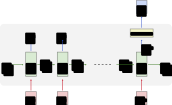
\includegraphics[width=0.8\textwidth]{figures/rnn_full}
    \caption{RNN Architecture known as Many-to-One \label{fig:rnn_architecture}}
    \vspace{-6pt}
\end{figure}

Figure~\ref{fig:rnn_architecture} shows the architecture of the model that we used, where
$T \in [0,15]$ (i.e., $1$ second per sample at $16Hz$), $S_t$ is called hidden state of the
RNN at time $t$ and it represents the information passed by the RNN at time $t-1$ to the RNN
at time $t$ (with $S_0$ set to $0$ and $S_T$ discarded), $Z_t$ is called output of the RNN
at time $t$, $X_t$ is the vector of features at time $t$ and contains $10$ features,
$Y \in [0,1,2,3]$ the output label indicating the activity that generated $X$.
The $SoftMax$ block converts
unnormalized logits returned by the last RNN into a probability distribution over classes.

We train our model using the Adam optimizer~\cite{kingma2014adam}.
The learning process is driven by the minimization of the cross-entropy loss
function~\cite{rubinstein1999cross}.

\subsection{Dataset}
\vspace{-.2cm}

We trained our model on $900$ samples of $16$ IMU readings each. We removed $144$ samples
from the training data and used it for testing our model and decide when to stop training.


\section{Results}
\vspace{-.3cm}

\t The accuracy of our recurrent neural network is very high. Having cut each trace into one-second samples, each epoch of training contained 1041 samples. After only 4 epochs of training, our training accuracy hit 100\% as well as our post-epoch testing accuracy. Of course, this varied throughout the 50-epoch training, but accuracy remained near-perfect through all epochs after 3. The inclusion of the first derivative of acceleration with respect to time raised the accuracy of our model by almost 25\%, as it allowed the RNN to access the shape of the acceleration readings. Included below in Figure 1 is a plot of per-trace accuracy over the 50 epochs, which shows the rate of cross-validation correctness for each epoch.

\begin{figure}[h]
    \centering
    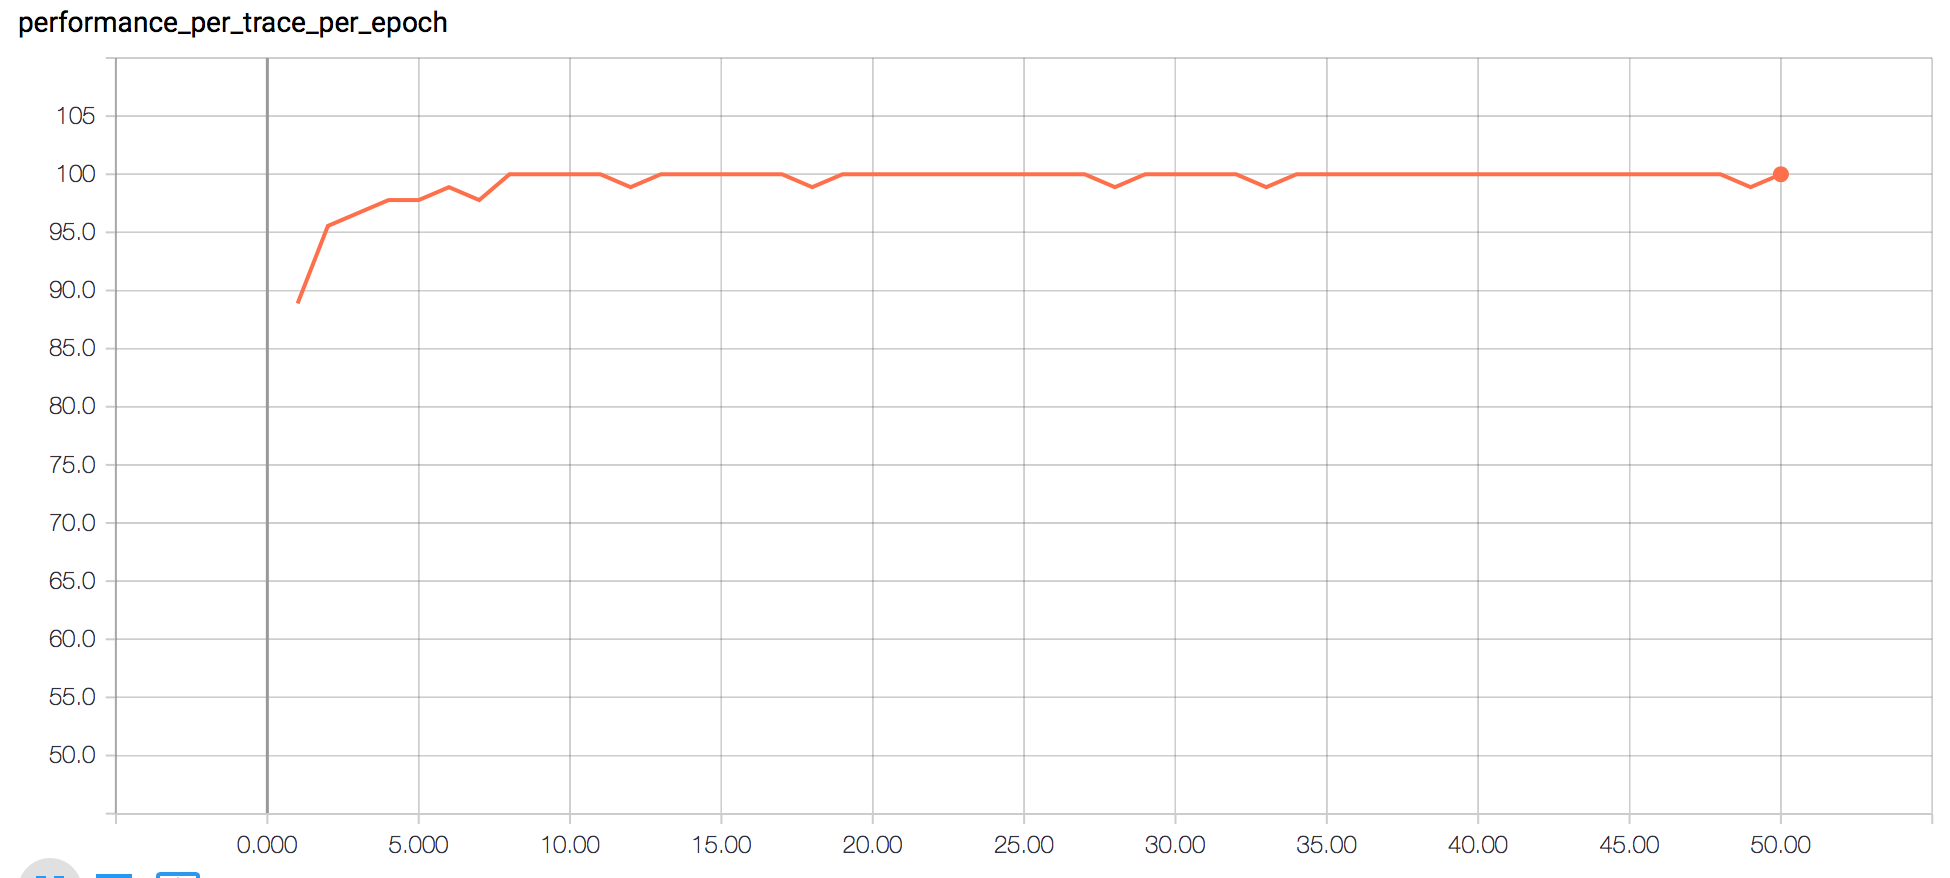
\includegraphics[width=0.7\linewidth]{figures/acc_ptpe.png}
    \caption{Accuracy per-trace per-epoch \label{fig:acc_ptpe}}
\end{figure}

\t Using held-out data, which is data that was not included in any of the training epochs, we observe testing accuracy of about 92\%, which is very high. The accuracy reduction is due to the model having difficulty distinguishing between standing and walking. We anticipate with more time and traces, this confusion will decrease as the model learns the subtle distinctions between the two activites. Shown below in Figure 2 is the corresponding confusion matrix for the final epoch using held-out data.

\begin{figure}[h]
    \centering
    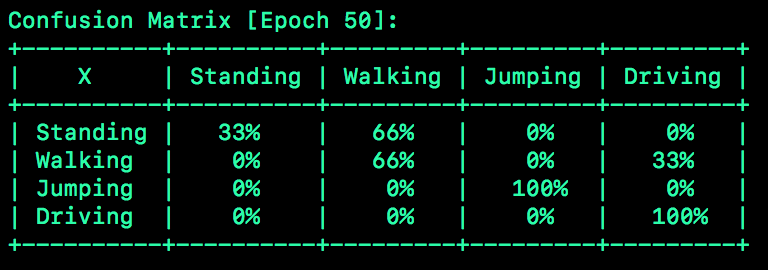
\includegraphics[width=0.8\linewidth]{figures/confusion.png}
    \caption{Confusion Matrix \label{fig:confusion}}
\end{figure}

\section{Conclusion}
\vspace{-.3cm}

\t Overall, this algorithm is very promising. It only relies on the reading of a sensor that is very popular in mobile devices, the IMU. After training, it requires very low CPU and battery usage for activity identification, and can be easily run in the background on many devices. Additionally, there exists extensive implementation of tensorflow for a variety of mobile devices. So, this algorithm can be deployed easily and seamlessly to mobile devices whether on a vehicle or on a smartphone. Expansion of this model to include more realistic identification classes, such as turning, would allow one to achieve accurate activity detection for many uses concerning safety and usability.


\bibliographystyle{abbrvnat}
{\scriptsize%
\bibliography{references}
}

\end{document}
